\documentclass{article}
\usepackage{tikz,lipsum,lmodern}
\usepackage[english]{babel}
\usepackage[most]{tcolorbox}
\usepackage[paperheight=10.75in,paperwidth=7.25in,margin=1in,heightrounded]{geometry}
\usepackage{graphicx}
\usepackage{blindtext}
\usepackage{ragged2e}
\usepackage{needspace}
\usepackage[space]{grffile}
\usepackage[utf8]{inputenc}
\usepackage[export]{adjustbox}
\usepackage{hyperref}
\usepackage{placeins}

\hypersetup{
    colorlinks,
    citecolor=black,
    filecolor=black,
    linkcolor=black,
    urlcolor=black
}
\usepackage{fancyhdr}
\pagestyle{fancy}
\fancyhf{}
\rhead{\rightmark}
\chead{\thepart}
\lhead{\nouppercase{\leftmark}}
\cfoot{\thepage}
\graphicspath{{"./img/"}}


\newcommand{\lbl}[1]{(see image \ref{#1}, \textit{\nameref{#1}})}

\title{%
Neural Networks \\
\large Deep Learning}

\author{Silas Hoffmann, inf103088}
\date{\today}


\begin{document}
\maketitle

\vspace{0.5cm}
\tableofcontents
\vspace{0.5cm}

\section{Introduction}
Notes for the introduction to neural networks presented by \textbf{3blue1brown}. Watch the whole series here: \href{https://www.youtube.com/watch?v=aircAruvnKk}. This series describes the strategy to recognize handwritten numbers.

\clearpage

\section{Chapter 1 - But what is a neural network?}


\subsection{Structural overview}

\FloatBarrier

\begin{figure}[h]
\centering
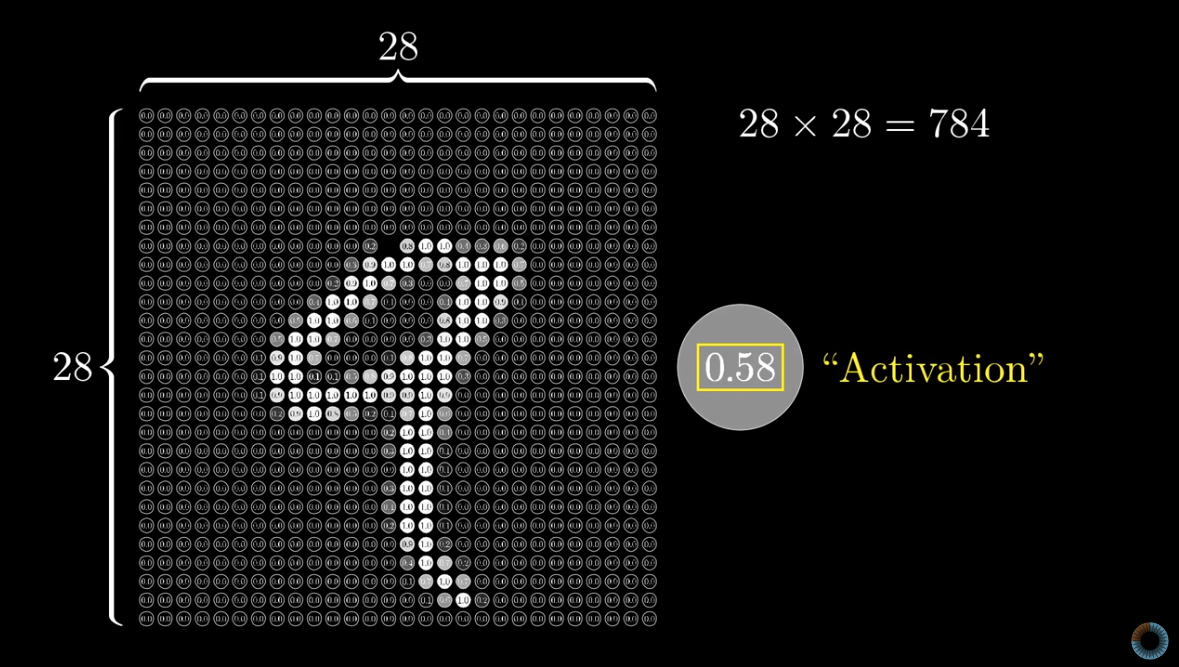
\includegraphics[max width=.9\textwidth]{ai_1.png}
\caption{Image interpreted as first layer of neural network}
\label{ai_1}
\end{figure}

Each pixel from the image is represented by a so called \textit{neuron} \lbl{ai_1}. These neurons possess a value called \textbf{Activiation} which contains a float between 0 and 1. This value specifies the brightness of this the particular pixel. This activation value also can be interpreted as how \textit{lit up} this particular neuron actually is, 1 meaning 100 \% in this context.


\begin{figure}[b!]
\centering
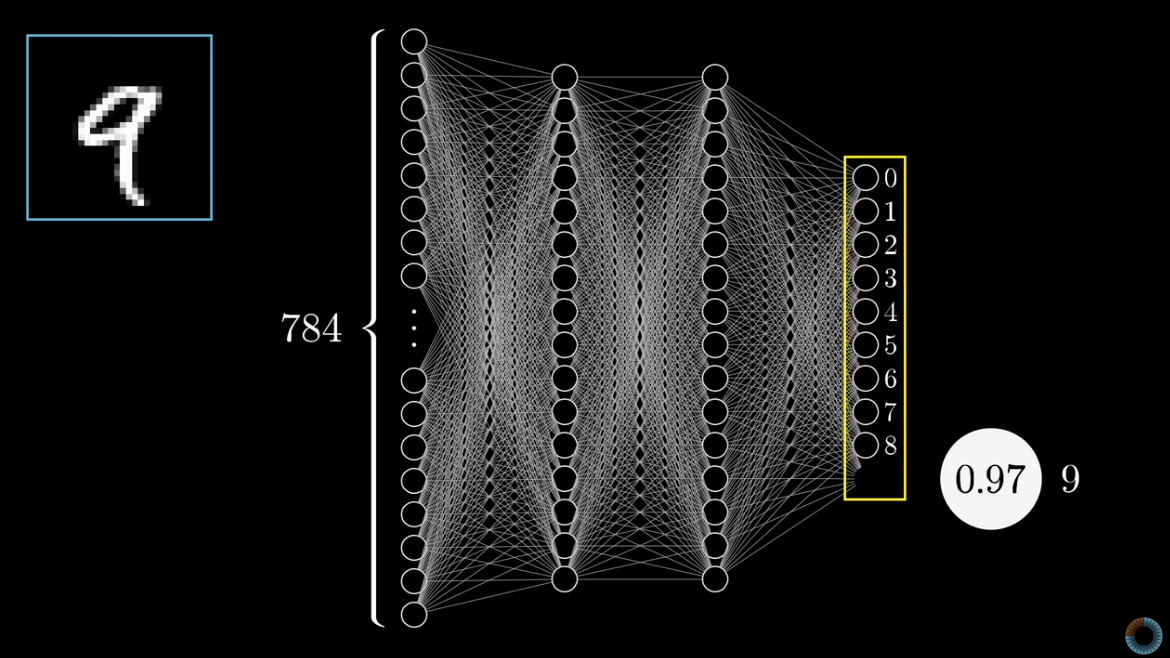
\includegraphics[max width=.9\textwidth]{ai_2.png}
\caption{Resulting top layer}
\label{ai_2}
\end{figure}

As each number is analyzed the top layer gives its prediction to a given input via Activation of the ten most right nodes \lbl{ai_2}. The one with the highest activation states what the system thinks the correct number might be. The layers between the top and the bottom layer are called \textbf{hidden layers}. 

\begin{figure}[h]
\centering
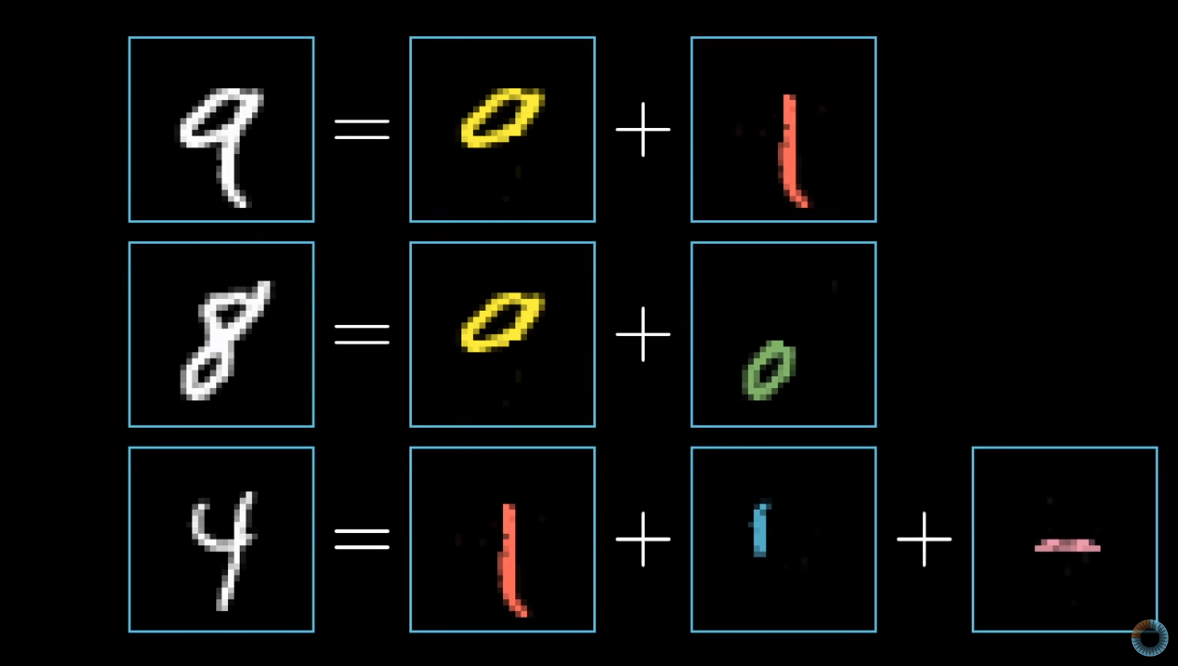
\includegraphics[max width=.9\textwidth]{ai_3.png}
\caption{Image interpreted as first layer of neural network}
\label{ai_3}
\end{figure}

The number of layers is not fixed and can be set to any number appropriate to the problem the system should solve. In this example it is useful to two hidden layers because of how the system works. A handwritten digit can be subdivided into different components \lbl{ai_3}. E.g. the number 9 can be divided into a top loop and a bottom line. These different steps will be analyzed by the various layers from the network. Maybe some digits share specific components and those nodes can be \textit{reused} \lbl{ai_4}. The idea is that any digit with a \textit{loopy} pattern towards the top sends of the specified neuron. This information is then used to fire up neurons in the next layer based on the idea that at least some kind of pattern already fits the input data.

\begin{figure}[h]
\centering
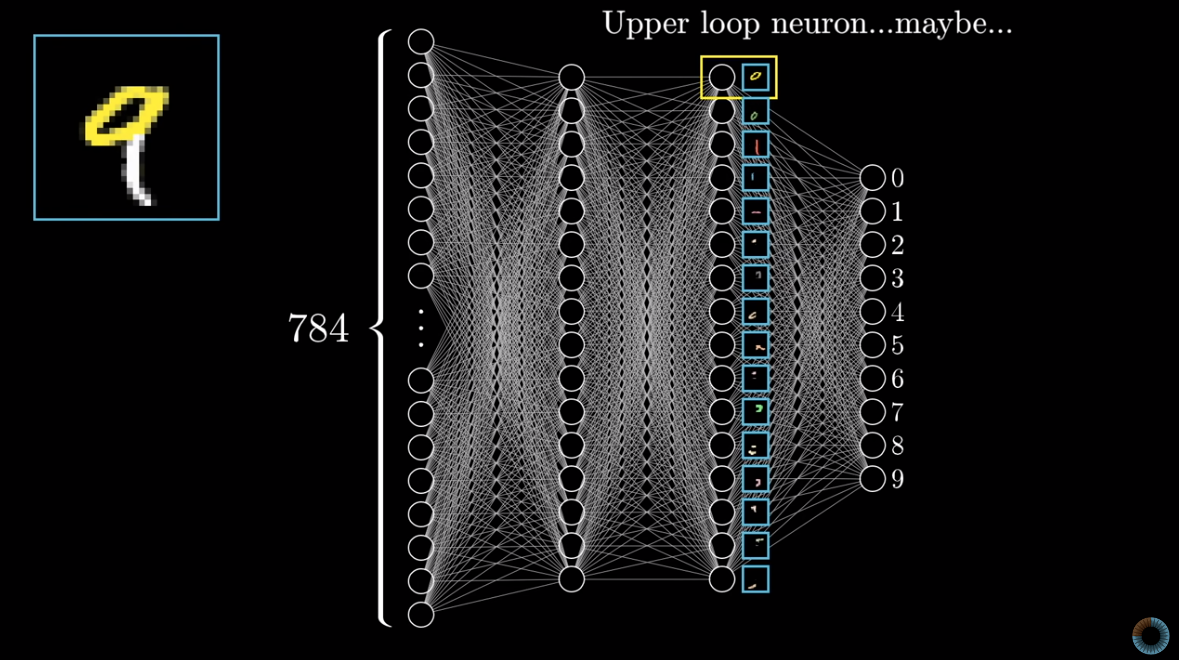
\includegraphics[max width=.9\textwidth]{ai_4.png}
\caption{Image interpreted as first layer of neural network}
\label{ai_4}
\end{figure}

But to be capable of recognizing such a complex patterns as a loop, the system has to recognize all the various subcomponents of a loop. Those mainly consist out of small edges which in total form a loop from a wider perspective. This may be the task of the second layer while the third layer is responsible for recognizing those more complex parts \lbl{ai_6}. 

Again, the number of layers is totally arbitrary. It might even be usefull to divide those smaller lines from layer 2 into smaller components, then there might be another layer. Or maybe the second layer is redundant altogether because the system can recognize those complex pattern directly. It always depends on the problem that the network should solve to decide how many layers are actually usefull.

\begin{figure}[h]
\centering
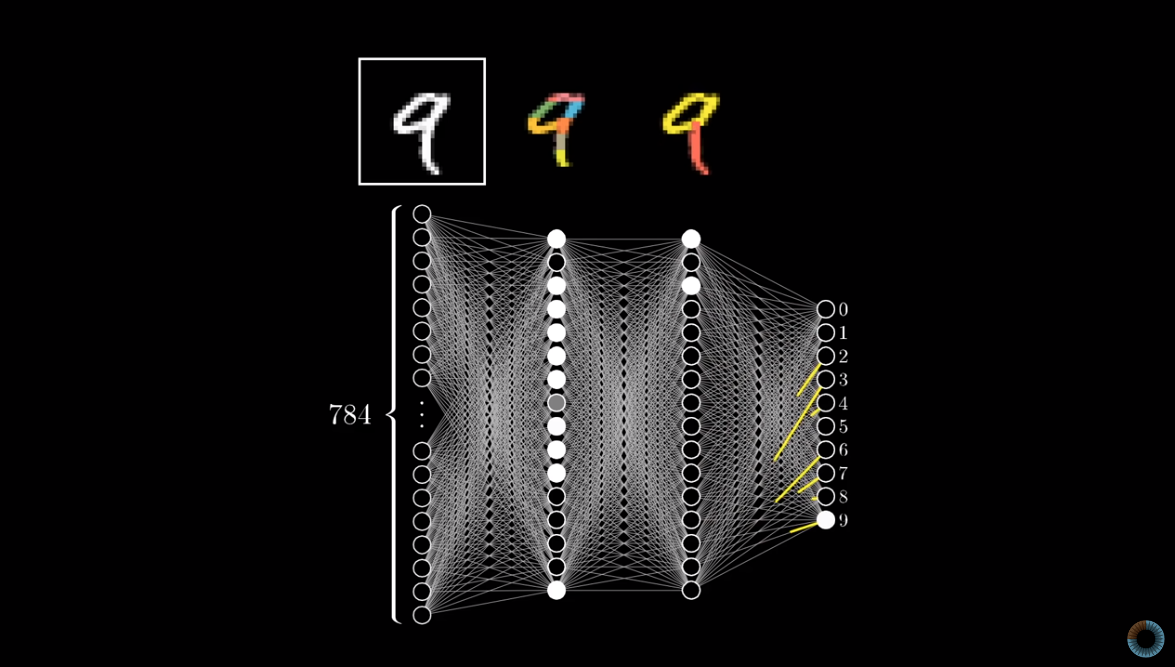
\includegraphics[max width=.9\textwidth]{ai_6.png}
\caption{Image interpreted as first layer of neural network}
\label{ai_6}
\end{figure}


\end{document}

